%%%%%%%%%%%%%%%%%%%%%%%%%%%%%%%%%%%%%%%%%
% Beamer Presentation
% LaTeX Template
% Version 1.0 (01/07/19)
%
%%%%%%%%%%%%%%%%%%%%%%%%%%%%%%%%%%%%%%%%%

%----------------------------------------------------------------
%	PACKAGES AND THEMES		-----------------------------------
%----------------------------------------------------------------

\documentclass[xcolor=table]{beamer}

\mode<presentation> {

\usetheme{Frankfurt}
\usecolortheme{dove}

}

\usepackage{graphicx}
\usepackage{booktabs} 
\usepackage{subfig}
\usepackage{pgf}
\usepackage{multirow}
\usepackage{appendixnumberbeamer}
\usepackage{bookmark}
\usepackage{siunitx}
\usepackage{animate}
\usepackage{xcolor}


%----------------------------------------------------------------
%	GENERAL OPTIONS 	-----------------------------------------
%----------------------------------------------------------------

% Set template options
\setbeamertemplate{section in toc}{\inserttocsectionnumber.~\inserttocsection}
\setbeamertemplate{frametitle}{\vspace*{1em}\insertframetitle}
\setbeamertemplate{enumerate items}[default]
\setbeamercolor{section in head/foot}{fg=white, bg=black}

% Headline
\makeatletter
\setbeamertemplate{headline}
{%
  \pgfuseshading{beamer@barshade}%
    \vskip-5ex%
  \begin{beamercolorbox}[ignorebg,ht=2.25ex,dp=3.75ex]{section in head/foot}
  \insertsectionnavigationhorizontal{\paperwidth}{\hskip0pt plus1fill}{\hskip0pt plus1fill}
  \end{beamercolorbox}%
  \ifbeamer@sb@subsection%
    \begin{beamercolorbox}[ignorebg,ht=2.125ex,dp=1.125ex,%
      leftskip=.3cm,rightskip=.3cm plus1fil]{subsection in head/foot}
      \usebeamerfont{subsection in head/foot}\insertsubsectionhead
    \end{beamercolorbox}%
  \fi%
}%
\makeatother

% Footline
\makeatletter
\setbeamertemplate{footline}
{
  \leavevmode%
  \hbox{%
  \begin{beamercolorbox}[wd=.333333\paperwidth,ht=2.25ex,dp=1ex,left]{section in head/foot}%
    \usebeamerfont{author in head/foot}\hspace{10pt}\insertshortauthor
  \end{beamercolorbox}%
  \begin{beamercolorbox}[wd=.333333\paperwidth,ht=2.25ex,dp=1ex,center]{section in head/foot}%
    \usebeamerfont{title in head/foot}\insertshorttitle
  \end{beamercolorbox}%
  \begin{beamercolorbox}[wd=.333333\paperwidth,ht=2.25ex,dp=1ex,right]{section in head/foot}%
    \usebeamerfont{date in head/foot}\insertshortdate{}\hspace*{2em}
    \insertframenumber{}\hspace*{2em}
  \end{beamercolorbox}}%
  \vskip0pt%
}
\makeatother

% Add logo
\logo{\pgfputat{\pgfxy(0,7)}{
\includegraphics[width=0.1\paperwidth]{Pictures/00_Unibe_Logo}}}

% Table settings
\renewcommand{\arraystretch}{2}
\captionsetup{labelformat=empty,labelsep=none}
\definecolor{Gray}{gray}{0.9}

%----------------------------------------------------------------
%	TITLE PAGE 	-------------------------------------------------
%----------------------------------------------------------------

\title[Regular Meeting]{
\uppercase{Regular Meeting}
} 

\author{Mathieu Simon}
\institute[University of Bern]
{
MSc - Biomedical Engineering \\
University of Bern, Faculty of Medicine \\
\medskip
}
\date{November 23, 2020}

\begin{document}

\begin{frame}
\titlepage
\end{frame}

	\begin{frame}
	\frametitle{Groups Distributions}
	\begin{columns}[c] 
		\column{.1\textwidth}
		\hspace{5mm}
		\rotatebox{90}{\hspace{5mm} OI group\hspace{8mm} Healthy group}
		\column{0.8\textwidth}
		\begin{figure}
			\hspace{-15mm}
			\captionsetup[subfigure]{labelformat=empty}
			\subfloat[]{
				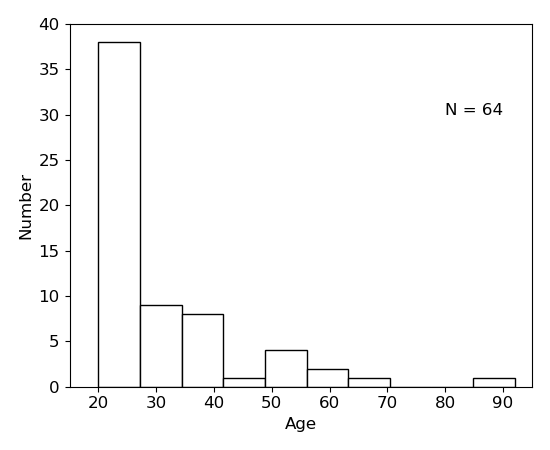
\includegraphics[width=0.4\linewidth]
				{Pictures/01_HealthyF}}
			\qquad
			\subfloat[]{
				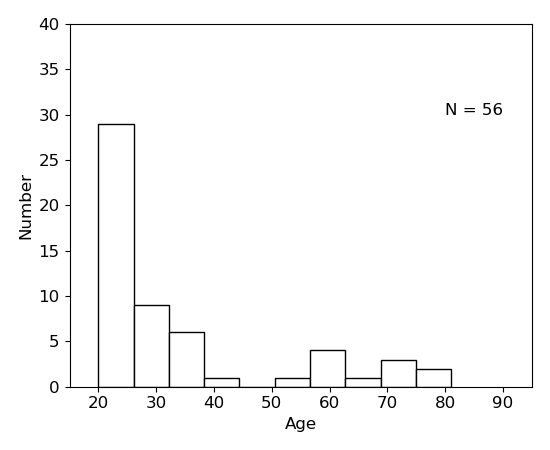
\includegraphics[width=0.4\linewidth]
				{Pictures/01_HealthyM}}
			\qquad\\
			\hspace{-15mm}
			\subfloat[Female]{
				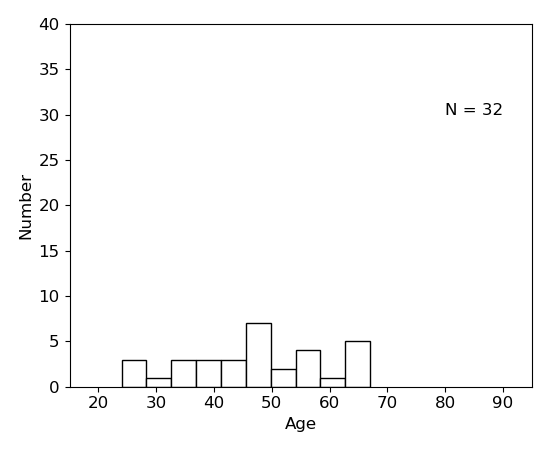
\includegraphics[width=0.4\linewidth,trim=0 0 0 100]
				{Pictures/01_OIF}}
			\qquad
			\subfloat[Male]{
				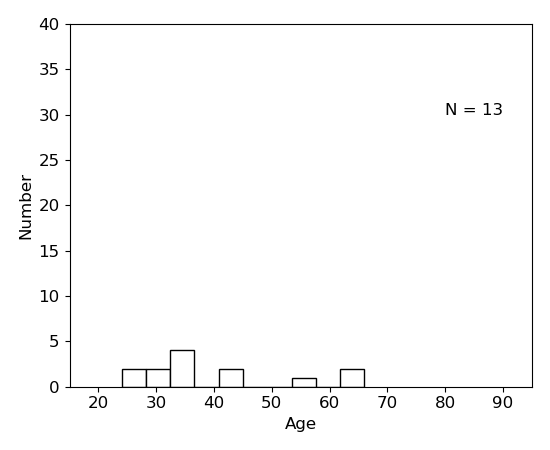
\includegraphics[width=0.4\linewidth,trim=0 0 0 100]
				{Pictures/01_OIM}}
		\end{figure}
	\end{columns}
\end{frame}

%----------------------------------------------------------------
%----------------------------------------------------------------
%----------------------------------------------------------------

\end{document} 